

% Formatting the presentation
% Change this file to change or remove the logo




% Specify sans body text, math serif text
\documentclass[sans, mathserif, professionalfont, 11pt]{beamer}

% \documentclass[sans]{beamer}

% \documentclass{beamer}

% Specify fonts
% \usepackage[default]{roboto}
% \usepackage[scaled]{helvet} % Sans sefif body text
\usepackage{txfonts}
\usepackage[scaled]{helvet} % Sans sefif body text
% \usepackage[]{comicneue} % Sans sefif body text
% \usepackage{cmbright}
% \usepackage[default]{comicneue}
% \usepackage{mathpazo} % Palatino for math
% \usepackage{eulervm}
\usepackage[scaled=0.95]{inconsolata} % Inconsolata fixed width font
% \usepackage[]{inconsolata} % Inconsolata fixed width font

% \usepackage[]{txfonts}

\usepackage{tikz}
\usepackage{ragged2e}
\usepackage{lipsum}
\usepackage{hyperref}

\justifying

% Bibliography
\usepackage[round]{natbib}
% \bibliographystyle{apacite}
\usepackage{appendixnumberbeamer}
\bibliographystyle{plainnat}
% \AtBeginDocument{\renewcommand{\harvardand}{\&}}

\newcommand\ind{\protect\mathpalette{\protect\independenT}{\perp}}
\def\independenT#1#2{\mathrel{\rlap{$#1#2$}\mkern2mu{#1#2}}}


\newcommand{\U}{\mathbf{U}}
\newcommand{\M}{\mathbf{M}}
\newcommand{\m}{\mathbf{m}}
\newcommand{\w}{\mathbf{w}}

\newcommand{\N}{\mathcal{N}}
\newcommand{\dee}{\mathrm{d}}
\newcommand{\F}{\mathcal{F}}
\newcommand{\trans}{\intercal}
\newcommand{\y}{\mathbf{y}}
\newcommand{\f}{\mathbf{f}}
\newcommand{\I}{\mathcal{I}}
\newcommand{\gammatilde}{\tilde{\gamma}}
\newcommand{\betabar}{\bar{\beta}}
\newcommand{\Ytilde}{\tilde{Y}}
\newcommand{\LL}{\mathcal{L}}
\newcommand{\E}{\mathrm{E}}


% Use mathbb symbols from Computer Modern
% \AtBeginDocument{
%   \DeclareSymbolFont{AMSb}{U}{msb}{m}{n}
%   \DeclareSymbolFontAlphabet{\mathbb}{AMSb}}

\DeclareMathOperator{\EE}{E}

% Graphics, tables, math, etc.
\usepackage{graphicx} 
\usepackage{booktabs} 
\usepackage{amsmath}
\usepackage{bm}
\usepackage{amssymb}
\usepackage{xcolor}

% \usepackage[symbol]{footmisc}

% \renewcommand{\thefootnote}{\fnsymbol{footnote}}

\renewcommand*{\thefootnote}{\fnsymbol{footnote}}

% Formatting
\setbeamertemplate{caption}[numbered]

\setbeamertemplate{title page}
{
  \begin{minipage}[b][\paperheight]{\textwidth}
    \vfill
    \ifx\inserttitle\@empty%
    \else%
    {\raggedright\linespread{0.8}\usebeamerfont{title}\usebeamercolor[fg]{title}
      % \scshape\MakeLowercase{\inserttitle}\par}%
      \scshape
      {\inserttitle}\par}%
    \vspace*{0.5em}
    \fi%
    \ifx\insertsubtitle\@empty%
    \else%
    {\usebeamerfont{subtitle}\usebeamercolor[fg]{subtitle}\insertsubtitle\par}%
    \vspace*{0.5em}
    \hrule
    \fi%
    \vspace*{0.5em}
    \ifx\insertauthor\@empty%
    \else%
    {\usebeamerfont{author}\usebeamercolor[fg]{author}\insertauthor\par}%
    \vspace*{0.25em}
    \fi%
    % Institute
    \ifx\insertinstitut\@empty%
    \else%
    \vspace*{3mm}
    {\usebeamerfont{institute}\usebeamercolor[fg]{institute}\insertinstitute\par}%
    \fi%
        \vspace*{3mm}
        % Date
    \ifx\insertdate\@empty%
    \else%
    {\usebeamerfont{date}\usebeamercolor[fg]{date}\insertdate\par}%
    \fi%
    \vspace*{5mm}
    % \vfill
    % -------------------------------------------------------------------------
    % -------------------------------------------------------------------------
    % -------------------------------------------------------------------------
    % -------------------------------------------------------------------------
    % University logo; if none, comment out
    \if1\graphic{
      % \begin{center}
      
\includegraphics[width=0.5\textwidth]{img/department-logo.png}\\
      % 
\includegraphics[width=0.6\textwidth]{img/McCombs_School_Brand_Branded.png}
      % 
\includegraphics[width=0.6\textwidth]{img/irom-logo.png}
      % \end{center}
    }\fi
    % -------------------------------------------------------------------------
    % -------------------------------------------------------------------------
    % -------------------------------------------------------------------------
    % -------------------------------------------------------------------------
  \vfill
  \vspace*{5mm}
  \end{minipage}
}

% \AtBeginSection{\frame{\sectionpage}}

\setbeamertemplate{frametitle}
  {\begin{flushleft}\smallskip 
    \insertframetitle\par 
   \vskip1pt\end{flushleft}}
\setbeamertemplate{itemize item}{$\bullet$}
\setbeamertemplate{navigation symbols}{}
% \setbeamertemplate{footline}[text line]{%
%     \hfill
% }
 \setbeamertemplate {footline}{\quad\hfill\insertframenumber\strut\quad}
\setbeamertemplate{footline}{
  \hfill%
  \usebeamercolor[fg]{page number in head/foot}%
  \usebeamerfont{page number in head/foot}%
  % Use this line for only the current frame number
  \setbeamertemplate{page number in head/foot}[framenumber]%
  % Use this line for frame number and *total* frame number
    % \setbeamertemplate{page number in head/foot}[totalframenumber]%
  \usebeamertemplate*{page number in head/foot}\kern1.5em\vskip8pt
}


% You can customize color settings here

% % Define some colors:

% Colors from R; see following page
% http://research.stowers.org/mcm/efg/R/Color/Chart/ColorChart.pdf
\definecolor{white}{HTML}{FFFFFF}
\definecolor{aliceblue}{HTML}{F0F8FF}
\definecolor{antiquewhite}{HTML}{FAEBD7}
\definecolor{antiquewhite1}{HTML}{FFEFDB}
\definecolor{antiquewhite2}{HTML}{EEDFCC}
\definecolor{antiquewhite3}{HTML}{CDC0B0}
\definecolor{antiquewhite4}{HTML}{8B8378}
\definecolor{aquamarine}{HTML}{7FFFD4}
\definecolor{aquamarine1}{HTML}{7FFFD4}
\definecolor{aquamarine2}{HTML}{76EEC6}
\definecolor{aquamarine3}{HTML}{66CDAA}
\definecolor{aquamarine4}{HTML}{458B74}
\definecolor{azure}{HTML}{F0FFFF}
\definecolor{azure1}{HTML}{F0FFFF}
\definecolor{azure2}{HTML}{E0EEEE}
\definecolor{azure3}{HTML}{C1CDCD}
\definecolor{azure4}{HTML}{838B8B}
\definecolor{beige}{HTML}{F5F5DC}
\definecolor{bisque}{HTML}{FFE4C4}
\definecolor{bisque1}{HTML}{FFE4C4}
\definecolor{bisque2}{HTML}{EED5B7}
\definecolor{bisque3}{HTML}{CDB79E}
\definecolor{bisque4}{HTML}{8B7D6B}
\definecolor{black}{HTML}{000000}
\definecolor{blanchedalmond}{HTML}{FFEBCD}
\definecolor{blue}{HTML}{0000FF}
\definecolor{blue1}{HTML}{0000FF}
\definecolor{blue2}{HTML}{0000EE}
\definecolor{blue3}{HTML}{0000CD}
\definecolor{blue4}{HTML}{00008B}
\definecolor{blueviolet}{HTML}{8A2BE2}
\definecolor{brown}{HTML}{A52A2A}
\definecolor{brown1}{HTML}{FF4040}
\definecolor{brown2}{HTML}{EE3B3B}
\definecolor{brown3}{HTML}{CD3333}
\definecolor{brown4}{HTML}{8B2323}
\definecolor{burlywood}{HTML}{DEB887}
\definecolor{burlywood1}{HTML}{FFD39B}
\definecolor{burlywood2}{HTML}{EEC591}
\definecolor{burlywood3}{HTML}{CDAA7D}
\definecolor{burlywood4}{HTML}{8B7355}
\definecolor{cadetblue}{HTML}{5F9EA0}
\definecolor{cadetblue1}{HTML}{98F5FF}
\definecolor{cadetblue2}{HTML}{8EE5EE}
\definecolor{cadetblue3}{HTML}{7AC5CD}
\definecolor{cadetblue4}{HTML}{53868B}
\definecolor{chartreuse}{HTML}{7FFF00}
\definecolor{chartreuse1}{HTML}{7FFF00}
\definecolor{chartreuse2}{HTML}{76EE00}
\definecolor{chartreuse3}{HTML}{66CD00}
\definecolor{chartreuse4}{HTML}{458B00}
\definecolor{chocolate}{HTML}{D2691E}
\definecolor{chocolate1}{HTML}{FF7F24}
\definecolor{chocolate2}{HTML}{EE7621}
\definecolor{chocolate3}{HTML}{CD661D}
\definecolor{chocolate4}{HTML}{8B4513}
\definecolor{coral}{HTML}{FF7F50}
\definecolor{coral1}{HTML}{FF7256}
\definecolor{coral2}{HTML}{EE6A50}
\definecolor{coral3}{HTML}{CD5B45}
\definecolor{coral4}{HTML}{8B3E2F}
\definecolor{cornflowerblue}{HTML}{6495ED}
\definecolor{cornsilk}{HTML}{FFF8DC}
\definecolor{cornsilk1}{HTML}{FFF8DC}
\definecolor{cornsilk2}{HTML}{EEE8CD}
\definecolor{cornsilk3}{HTML}{CDC8B1}
\definecolor{cornsilk4}{HTML}{8B8878}
\definecolor{cyan}{HTML}{00FFFF}
\definecolor{cyan1}{HTML}{00FFFF}
\definecolor{cyan2}{HTML}{00EEEE}
\definecolor{cyan3}{HTML}{00CDCD}
\definecolor{cyan4}{HTML}{008B8B}
\definecolor{darkblue}{HTML}{00008B}
\definecolor{darkcyan}{HTML}{008B8B}
\definecolor{darkgoldenrod}{HTML}{B8860B}
\definecolor{darkgoldenrod1}{HTML}{FFB90F}
\definecolor{darkgoldenrod2}{HTML}{EEAD0E}
\definecolor{darkgoldenrod3}{HTML}{CD950C}
\definecolor{darkgoldenrod4}{HTML}{8B6508}
\definecolor{darkgray}{HTML}{A9A9A9}
\definecolor{darkgreen}{HTML}{006400}
\definecolor{darkgrey}{HTML}{A9A9A9}
\definecolor{darkkhaki}{HTML}{BDB76B}
\definecolor{darkmagenta}{HTML}{8B008B}
\definecolor{darkolivegreen}{HTML}{556B2F}
\definecolor{darkolivegreen1}{HTML}{CAFF70}
\definecolor{darkolivegreen2}{HTML}{BCEE68}
\definecolor{darkolivegreen3}{HTML}{A2CD5A}
\definecolor{darkolivegreen4}{HTML}{6E8B3D}
\definecolor{darkorange}{HTML}{FF8C00}
\definecolor{darkorange1}{HTML}{FF7F00}
\definecolor{darkorange2}{HTML}{EE7600}
\definecolor{darkorange3}{HTML}{CD6600}
\definecolor{darkorange4}{HTML}{8B4500}
\definecolor{darkorchid}{HTML}{9932CC}
\definecolor{darkorchid1}{HTML}{BF3EFF}
\definecolor{darkorchid2}{HTML}{B23AEE}
\definecolor{darkorchid3}{HTML}{9A32CD}
\definecolor{darkorchid4}{HTML}{68228B}
\definecolor{darkred}{HTML}{8B0000}
\definecolor{darksalmon}{HTML}{E9967A}
\definecolor{darkseagreen}{HTML}{8FBC8F}
\definecolor{darkseagreen1}{HTML}{C1FFC1}
\definecolor{darkseagreen2}{HTML}{B4EEB4}
\definecolor{darkseagreen3}{HTML}{9BCD9B}
\definecolor{darkseagreen4}{HTML}{698B69}
\definecolor{darkslateblue}{HTML}{483D8B}
\definecolor{darkslategray}{HTML}{2F4F4F}
\definecolor{darkslategray1}{HTML}{97FFFF}
\definecolor{darkslategray2}{HTML}{8DEEEE}
\definecolor{darkslategray3}{HTML}{79CDCD}
\definecolor{darkslategray4}{HTML}{528B8B}
\definecolor{darkslategrey}{HTML}{2F4F4F}
\definecolor{darkturquoise}{HTML}{00CED1}
\definecolor{darkviolet}{HTML}{9400D3}
\definecolor{deeppink}{HTML}{FF1493}
\definecolor{deeppink1}{HTML}{FF1493}
\definecolor{deeppink2}{HTML}{EE1289}
\definecolor{deeppink3}{HTML}{CD1076}
\definecolor{deeppink4}{HTML}{8B0A50}
\definecolor{deepskyblue}{HTML}{00BFFF}
\definecolor{deepskyblue1}{HTML}{00BFFF}
\definecolor{deepskyblue2}{HTML}{00B2EE}
\definecolor{deepskyblue3}{HTML}{009ACD}
\definecolor{deepskyblue4}{HTML}{00688B}
\definecolor{dimgray}{HTML}{696969}
\definecolor{dimgrey}{HTML}{696969}
\definecolor{dodgerblue}{HTML}{1E90FF}
\definecolor{dodgerblue1}{HTML}{1E90FF}
\definecolor{dodgerblue2}{HTML}{1C86EE}
\definecolor{dodgerblue3}{HTML}{1874CD}
\definecolor{dodgerblue4}{HTML}{104E8B}
\definecolor{firebrick}{HTML}{B22222}
\definecolor{firebrick1}{HTML}{FF3030}
\definecolor{firebrick2}{HTML}{EE2C2C}
\definecolor{firebrick3}{HTML}{CD2626}
\definecolor{firebrick4}{HTML}{8B1A1A}
\definecolor{floralwhite}{HTML}{FFFAF0}
\definecolor{forestgreen}{HTML}{228B22}
\definecolor{gainsboro}{HTML}{DCDCDC}
\definecolor{ghostwhite}{HTML}{F8F8FF}
\definecolor{gold}{HTML}{FFD700}
\definecolor{gold1}{HTML}{FFD700}
\definecolor{gold2}{HTML}{EEC900}
\definecolor{gold3}{HTML}{CDAD00}
\definecolor{gold4}{HTML}{8B7500}
\definecolor{goldenrod}{HTML}{DAA520}
\definecolor{goldenrod1}{HTML}{FFC125}
\definecolor{goldenrod2}{HTML}{EEB422}
\definecolor{goldenrod3}{HTML}{CD9B1D}
\definecolor{goldenrod4}{HTML}{8B6914}
\definecolor{gray}{HTML}{BEBEBE}
\definecolor{gray0}{HTML}{000000}
\definecolor{gray1}{HTML}{030303}
\definecolor{gray2}{HTML}{050505}
\definecolor{gray3}{HTML}{080808}
\definecolor{gray4}{HTML}{0A0A0A}
\definecolor{gray5}{HTML}{0D0D0D}
\definecolor{gray6}{HTML}{0F0F0F}
\definecolor{gray7}{HTML}{121212}
\definecolor{gray8}{HTML}{141414}
\definecolor{gray9}{HTML}{171717}
\definecolor{gray10}{HTML}{1A1A1A}
\definecolor{gray11}{HTML}{1C1C1C}
\definecolor{gray12}{HTML}{1F1F1F}
\definecolor{gray13}{HTML}{212121}
\definecolor{gray14}{HTML}{242424}
\definecolor{gray15}{HTML}{262626}
\definecolor{gray16}{HTML}{292929}
\definecolor{gray17}{HTML}{2B2B2B}
\definecolor{gray18}{HTML}{2E2E2E}
\definecolor{gray19}{HTML}{303030}
\definecolor{gray20}{HTML}{333333}
\definecolor{gray21}{HTML}{363636}
\definecolor{gray22}{HTML}{383838}
\definecolor{gray23}{HTML}{3B3B3B}
\definecolor{gray24}{HTML}{3D3D3D}
\definecolor{gray25}{HTML}{404040}
\definecolor{gray26}{HTML}{424242}
\definecolor{gray27}{HTML}{454545}
\definecolor{gray28}{HTML}{474747}
\definecolor{gray29}{HTML}{4A4A4A}
\definecolor{gray30}{HTML}{4D4D4D}
\definecolor{gray31}{HTML}{4F4F4F}
\definecolor{gray32}{HTML}{525252}
\definecolor{gray33}{HTML}{545454}
\definecolor{gray34}{HTML}{575757}
\definecolor{gray35}{HTML}{595959}
\definecolor{gray36}{HTML}{5C5C5C}
\definecolor{gray37}{HTML}{5E5E5E}
\definecolor{gray38}{HTML}{616161}
\definecolor{gray39}{HTML}{636363}
\definecolor{gray40}{HTML}{666666}
\definecolor{gray41}{HTML}{696969}
\definecolor{gray42}{HTML}{6B6B6B}
\definecolor{gray43}{HTML}{6E6E6E}
\definecolor{gray44}{HTML}{707070}
\definecolor{gray45}{HTML}{737373}
\definecolor{gray46}{HTML}{757575}
\definecolor{gray47}{HTML}{787878}
\definecolor{gray48}{HTML}{7A7A7A}
\definecolor{gray49}{HTML}{7D7D7D}
\definecolor{gray50}{HTML}{7F7F7F}
\definecolor{gray51}{HTML}{828282}
\definecolor{gray52}{HTML}{858585}
\definecolor{gray53}{HTML}{878787}
\definecolor{gray54}{HTML}{8A8A8A}
\definecolor{gray55}{HTML}{8C8C8C}
\definecolor{gray56}{HTML}{8F8F8F}
\definecolor{gray57}{HTML}{919191}
\definecolor{gray58}{HTML}{949494}
\definecolor{gray59}{HTML}{969696}
\definecolor{gray60}{HTML}{999999}
\definecolor{gray61}{HTML}{9C9C9C}
\definecolor{gray62}{HTML}{9E9E9E}
\definecolor{gray63}{HTML}{A1A1A1}
\definecolor{gray64}{HTML}{A3A3A3}
\definecolor{gray65}{HTML}{A6A6A6}
\definecolor{gray66}{HTML}{A8A8A8}
\definecolor{gray67}{HTML}{ABABAB}
\definecolor{gray68}{HTML}{ADADAD}
\definecolor{gray69}{HTML}{B0B0B0}
\definecolor{gray70}{HTML}{B3B3B3}
\definecolor{gray71}{HTML}{B5B5B5}
\definecolor{gray72}{HTML}{B8B8B8}
\definecolor{gray73}{HTML}{BABABA}
\definecolor{gray74}{HTML}{BDBDBD}
\definecolor{gray75}{HTML}{BFBFBF}
\definecolor{gray76}{HTML}{C2C2C2}
\definecolor{gray77}{HTML}{C4C4C4}
\definecolor{gray78}{HTML}{C7C7C7}
\definecolor{gray79}{HTML}{C9C9C9}
\definecolor{gray80}{HTML}{CCCCCC}
\definecolor{gray81}{HTML}{CFCFCF}
\definecolor{gray82}{HTML}{D1D1D1}
\definecolor{gray83}{HTML}{D4D4D4}
\definecolor{gray84}{HTML}{D6D6D6}
\definecolor{gray85}{HTML}{D9D9D9}
\definecolor{gray86}{HTML}{DBDBDB}
\definecolor{gray87}{HTML}{DEDEDE}
\definecolor{gray88}{HTML}{E0E0E0}
\definecolor{gray89}{HTML}{E3E3E3}
\definecolor{gray90}{HTML}{E5E5E5}
\definecolor{gray91}{HTML}{E8E8E8}
\definecolor{gray92}{HTML}{EBEBEB}
\definecolor{gray93}{HTML}{EDEDED}
\definecolor{gray94}{HTML}{F0F0F0}
\definecolor{gray95}{HTML}{F2F2F2}
\definecolor{gray96}{HTML}{F5F5F5}
\definecolor{gray97}{HTML}{F7F7F7}
\definecolor{gray98}{HTML}{FAFAFA}
\definecolor{gray99}{HTML}{FCFCFC}
\definecolor{gray100}{HTML}{FFFFFF}
\definecolor{green}{HTML}{00FF00}
\definecolor{green1}{HTML}{00FF00}
\definecolor{green2}{HTML}{00EE00}
\definecolor{green3}{HTML}{00CD00}
\definecolor{green4}{HTML}{008B00}
\definecolor{greenyellow}{HTML}{ADFF2F}
\definecolor{grey}{HTML}{BEBEBE}
\definecolor{grey0}{HTML}{000000}
\definecolor{grey1}{HTML}{030303}
\definecolor{grey2}{HTML}{050505}
\definecolor{grey3}{HTML}{080808}
\definecolor{grey4}{HTML}{0A0A0A}
\definecolor{grey5}{HTML}{0D0D0D}
\definecolor{grey6}{HTML}{0F0F0F}
\definecolor{grey7}{HTML}{121212}
\definecolor{grey8}{HTML}{141414}
\definecolor{grey9}{HTML}{171717}
\definecolor{grey10}{HTML}{1A1A1A}
\definecolor{grey11}{HTML}{1C1C1C}
\definecolor{grey12}{HTML}{1F1F1F}
\definecolor{grey13}{HTML}{212121}
\definecolor{grey14}{HTML}{242424}
\definecolor{grey15}{HTML}{262626}
\definecolor{grey16}{HTML}{292929}
\definecolor{grey17}{HTML}{2B2B2B}
\definecolor{grey18}{HTML}{2E2E2E}
\definecolor{grey19}{HTML}{303030}
\definecolor{grey20}{HTML}{333333}
\definecolor{grey21}{HTML}{363636}
\definecolor{grey22}{HTML}{383838}
\definecolor{grey23}{HTML}{3B3B3B}
\definecolor{grey24}{HTML}{3D3D3D}
\definecolor{grey25}{HTML}{404040}
\definecolor{grey26}{HTML}{424242}
\definecolor{grey27}{HTML}{454545}
\definecolor{grey28}{HTML}{474747}
\definecolor{grey29}{HTML}{4A4A4A}
\definecolor{grey30}{HTML}{4D4D4D}
\definecolor{grey31}{HTML}{4F4F4F}
\definecolor{grey32}{HTML}{525252}
\definecolor{grey33}{HTML}{545454}
\definecolor{grey34}{HTML}{575757}
\definecolor{grey35}{HTML}{595959}
\definecolor{grey36}{HTML}{5C5C5C}
\definecolor{grey37}{HTML}{5E5E5E}
\definecolor{grey38}{HTML}{616161}
\definecolor{grey39}{HTML}{636363}
\definecolor{grey40}{HTML}{666666}
\definecolor{grey41}{HTML}{696969}
\definecolor{grey42}{HTML}{6B6B6B}
\definecolor{grey43}{HTML}{6E6E6E}
\definecolor{grey44}{HTML}{707070}
\definecolor{grey45}{HTML}{737373}
\definecolor{grey46}{HTML}{757575}
\definecolor{grey47}{HTML}{787878}
\definecolor{grey48}{HTML}{7A7A7A}
\definecolor{grey49}{HTML}{7D7D7D}
\definecolor{grey50}{HTML}{7F7F7F}
\definecolor{grey51}{HTML}{828282}
\definecolor{grey52}{HTML}{858585}
\definecolor{grey53}{HTML}{878787}
\definecolor{grey54}{HTML}{8A8A8A}
\definecolor{grey55}{HTML}{8C8C8C}
\definecolor{grey56}{HTML}{8F8F8F}
\definecolor{grey57}{HTML}{919191}
\definecolor{grey58}{HTML}{949494}
\definecolor{grey59}{HTML}{969696}
\definecolor{grey60}{HTML}{999999}
\definecolor{grey61}{HTML}{9C9C9C}
\definecolor{grey62}{HTML}{9E9E9E}
\definecolor{grey63}{HTML}{A1A1A1}
\definecolor{grey64}{HTML}{A3A3A3}
\definecolor{grey65}{HTML}{A6A6A6}
\definecolor{grey66}{HTML}{A8A8A8}
\definecolor{grey67}{HTML}{ABABAB}
\definecolor{grey68}{HTML}{ADADAD}
\definecolor{grey69}{HTML}{B0B0B0}
\definecolor{grey70}{HTML}{B3B3B3}
\definecolor{grey71}{HTML}{B5B5B5}
\definecolor{grey72}{HTML}{B8B8B8}
\definecolor{grey73}{HTML}{BABABA}
\definecolor{grey74}{HTML}{BDBDBD}
\definecolor{grey75}{HTML}{BFBFBF}
\definecolor{grey76}{HTML}{C2C2C2}
\definecolor{grey77}{HTML}{C4C4C4}
\definecolor{grey78}{HTML}{C7C7C7}
\definecolor{grey79}{HTML}{C9C9C9}
\definecolor{grey80}{HTML}{CCCCCC}
\definecolor{grey81}{HTML}{CFCFCF}
\definecolor{grey82}{HTML}{D1D1D1}
\definecolor{grey83}{HTML}{D4D4D4}
\definecolor{grey84}{HTML}{D6D6D6}
\definecolor{grey85}{HTML}{D9D9D9}
\definecolor{grey86}{HTML}{DBDBDB}
\definecolor{grey87}{HTML}{DEDEDE}
\definecolor{grey88}{HTML}{E0E0E0}
\definecolor{grey89}{HTML}{E3E3E3}
\definecolor{grey90}{HTML}{E5E5E5}
\definecolor{grey91}{HTML}{E8E8E8}
\definecolor{grey92}{HTML}{EBEBEB}
\definecolor{grey93}{HTML}{EDEDED}
\definecolor{grey94}{HTML}{F0F0F0}
\definecolor{grey95}{HTML}{F2F2F2}
\definecolor{grey96}{HTML}{F5F5F5}
\definecolor{grey97}{HTML}{F7F7F7}
\definecolor{grey98}{HTML}{FAFAFA}
\definecolor{grey99}{HTML}{FCFCFC}
\definecolor{grey100}{HTML}{FFFFFF}
\definecolor{honeydew}{HTML}{F0FFF0}
\definecolor{honeydew1}{HTML}{F0FFF0}
\definecolor{honeydew2}{HTML}{E0EEE0}
\definecolor{honeydew3}{HTML}{C1CDC1}
\definecolor{honeydew4}{HTML}{838B83}
\definecolor{hotpink}{HTML}{FF69B4}
\definecolor{hotpink1}{HTML}{FF6EB4}
\definecolor{hotpink2}{HTML}{EE6AA7}
\definecolor{hotpink3}{HTML}{CD6090}
\definecolor{hotpink4}{HTML}{8B3A62}
\definecolor{indianred}{HTML}{CD5C5C}
\definecolor{indianred1}{HTML}{FF6A6A}
\definecolor{indianred2}{HTML}{EE6363}
\definecolor{indianred3}{HTML}{CD5555}
\definecolor{indianred4}{HTML}{8B3A3A}
\definecolor{ivory}{HTML}{FFFFF0}
\definecolor{ivory1}{HTML}{FFFFF0}
\definecolor{ivory2}{HTML}{EEEEE0}
\definecolor{ivory3}{HTML}{CDCDC1}
\definecolor{ivory4}{HTML}{8B8B83}
\definecolor{khaki}{HTML}{F0E68C}
\definecolor{khaki1}{HTML}{FFF68F}
\definecolor{khaki2}{HTML}{EEE685}
\definecolor{khaki3}{HTML}{CDC673}
\definecolor{khaki4}{HTML}{8B864E}
\definecolor{lavender}{HTML}{E6E6FA}
\definecolor{lavenderblush}{HTML}{FFF0F5}
\definecolor{lavenderblush1}{HTML}{FFF0F5}
\definecolor{lavenderblush2}{HTML}{EEE0E5}
\definecolor{lavenderblush3}{HTML}{CDC1C5}
\definecolor{lavenderblush4}{HTML}{8B8386}
\definecolor{lawngreen}{HTML}{7CFC00}
\definecolor{lemonchiffon}{HTML}{FFFACD}
\definecolor{lemonchiffon1}{HTML}{FFFACD}
\definecolor{lemonchiffon2}{HTML}{EEE9BF}
\definecolor{lemonchiffon3}{HTML}{CDC9A5}
\definecolor{lemonchiffon4}{HTML}{8B8970}
\definecolor{lightblue}{HTML}{ADD8E6}
\definecolor{lightblue1}{HTML}{BFEFFF}
\definecolor{lightblue2}{HTML}{B2DFEE}
\definecolor{lightblue3}{HTML}{9AC0CD}
\definecolor{lightblue4}{HTML}{68838B}
\definecolor{lightcoral}{HTML}{F08080}
\definecolor{lightcyan}{HTML}{E0FFFF}
\definecolor{lightcyan1}{HTML}{E0FFFF}
\definecolor{lightcyan2}{HTML}{D1EEEE}
\definecolor{lightcyan3}{HTML}{B4CDCD}
\definecolor{lightcyan4}{HTML}{7A8B8B}
\definecolor{lightgoldenrod}{HTML}{EEDD82}
\definecolor{lightgoldenrod1}{HTML}{FFEC8B}
\definecolor{lightgoldenrod2}{HTML}{EEDC82}
\definecolor{lightgoldenrod3}{HTML}{CDBE70}
\definecolor{lightgoldenrod4}{HTML}{8B814C}
\definecolor{lightgoldenrodyellow}{HTML}{FAFAD2}
\definecolor{lightgray}{HTML}{D3D3D3}
\definecolor{lightgreen}{HTML}{90EE90}
\definecolor{lightgrey}{HTML}{D3D3D3}
\definecolor{lightpink}{HTML}{FFB6C1}
\definecolor{lightpink1}{HTML}{FFAEB9}
\definecolor{lightpink2}{HTML}{EEA2AD}
\definecolor{lightpink3}{HTML}{CD8C95}
\definecolor{lightpink4}{HTML}{8B5F65}
\definecolor{lightsalmon}{HTML}{FFA07A}
\definecolor{lightsalmon1}{HTML}{FFA07A}
\definecolor{lightsalmon2}{HTML}{EE9572}
\definecolor{lightsalmon3}{HTML}{CD8162}
\definecolor{lightsalmon4}{HTML}{8B5742}
\definecolor{lightseagreen}{HTML}{20B2AA}
\definecolor{lightskyblue}{HTML}{87CEFA}
\definecolor{lightskyblue1}{HTML}{B0E2FF}
\definecolor{lightskyblue2}{HTML}{A4D3EE}
\definecolor{lightskyblue3}{HTML}{8DB6CD}
\definecolor{lightskyblue4}{HTML}{607B8B}
\definecolor{lightslateblue}{HTML}{8470FF}
\definecolor{lightslategray}{HTML}{778899}
\definecolor{lightslategrey}{HTML}{778899}
\definecolor{lightsteelblue}{HTML}{B0C4DE}
\definecolor{lightsteelblue1}{HTML}{CAE1FF}
\definecolor{lightsteelblue2}{HTML}{BCD2EE}
\definecolor{lightsteelblue3}{HTML}{A2B5CD}
\definecolor{lightsteelblue4}{HTML}{6E7B8B}
\definecolor{lightyellow}{HTML}{FFFFE0}
\definecolor{lightyellow1}{HTML}{FFFFE0}
\definecolor{lightyellow2}{HTML}{EEEED1}
\definecolor{lightyellow3}{HTML}{CDCDB4}
\definecolor{lightyellow4}{HTML}{8B8B7A}
\definecolor{limegreen}{HTML}{32CD32}
\definecolor{linen}{HTML}{FAF0E6}
\definecolor{magenta}{HTML}{FF00FF}
\definecolor{magenta1}{HTML}{FF00FF}
\definecolor{magenta2}{HTML}{EE00EE}
\definecolor{magenta3}{HTML}{CD00CD}
\definecolor{magenta4}{HTML}{8B008B}
\definecolor{maroon}{HTML}{B03060}
\definecolor{maroon1}{HTML}{FF34B3}
\definecolor{maroon2}{HTML}{EE30A7}
\definecolor{maroon3}{HTML}{CD2990}
\definecolor{maroon4}{HTML}{8B1C62}
\definecolor{mediumaquamarine}{HTML}{66CDAA}
\definecolor{mediumblue}{HTML}{0000CD}
\definecolor{mediumorchid}{HTML}{BA55D3}
\definecolor{mediumorchid1}{HTML}{E066FF}
\definecolor{mediumorchid2}{HTML}{D15FEE}
\definecolor{mediumorchid3}{HTML}{B452CD}
\definecolor{mediumorchid4}{HTML}{7A378B}
\definecolor{mediumpurple}{HTML}{9370DB}
\definecolor{mediumpurple1}{HTML}{AB82FF}
\definecolor{mediumpurple2}{HTML}{9F79EE}
\definecolor{mediumpurple3}{HTML}{8968CD}
\definecolor{mediumpurple4}{HTML}{5D478B}
\definecolor{mediumseagreen}{HTML}{3CB371}
\definecolor{mediumslateblue}{HTML}{7B68EE}
\definecolor{mediumspringgreen}{HTML}{00FA9A}
\definecolor{mediumturquoise}{HTML}{48D1CC}
\definecolor{mediumvioletred}{HTML}{C71585}
\definecolor{midnightblue}{HTML}{191970}
\definecolor{mintcream}{HTML}{F5FFFA}
\definecolor{mistyrose}{HTML}{FFE4E1}
\definecolor{mistyrose1}{HTML}{FFE4E1}
\definecolor{mistyrose2}{HTML}{EED5D2}
\definecolor{mistyrose3}{HTML}{CDB7B5}
\definecolor{mistyrose4}{HTML}{8B7D7B}
\definecolor{moccasin}{HTML}{FFE4B5}
\definecolor{navajowhite}{HTML}{FFDEAD}
\definecolor{navajowhite1}{HTML}{FFDEAD}
\definecolor{navajowhite2}{HTML}{EECFA1}
\definecolor{navajowhite3}{HTML}{CDB38B}
\definecolor{navajowhite4}{HTML}{8B795E}
\definecolor{navy}{HTML}{000080}
\definecolor{navyblue}{HTML}{000080}
\definecolor{oldlace}{HTML}{FDF5E6}
\definecolor{olivedrab}{HTML}{6B8E23}
\definecolor{olivedrab1}{HTML}{C0FF3E}
\definecolor{olivedrab2}{HTML}{B3EE3A}
\definecolor{olivedrab3}{HTML}{9ACD32}
\definecolor{olivedrab4}{HTML}{698B22}
\definecolor{orange}{HTML}{FFA500}
\definecolor{orange1}{HTML}{FFA500}
\definecolor{orange2}{HTML}{EE9A00}
\definecolor{orange3}{HTML}{CD8500}
\definecolor{orange4}{HTML}{8B5A00}
\definecolor{orangered}{HTML}{FF4500}
\definecolor{orangered1}{HTML}{FF4500}
\definecolor{orangered2}{HTML}{EE4000}
\definecolor{orangered3}{HTML}{CD3700}
\definecolor{orangered4}{HTML}{8B2500}
\definecolor{orchid}{HTML}{DA70D6}
\definecolor{orchid1}{HTML}{FF83FA}
\definecolor{orchid2}{HTML}{EE7AE9}
\definecolor{orchid3}{HTML}{CD69C9}
\definecolor{orchid4}{HTML}{8B4789}
\definecolor{palegoldenrod}{HTML}{EEE8AA}
\definecolor{palegreen}{HTML}{98FB98}
\definecolor{palegreen1}{HTML}{9AFF9A}
\definecolor{palegreen2}{HTML}{90EE90}
\definecolor{palegreen3}{HTML}{7CCD7C}
\definecolor{palegreen4}{HTML}{548B54}
\definecolor{paleturquoise}{HTML}{AFEEEE}
\definecolor{paleturquoise1}{HTML}{BBFFFF}
\definecolor{paleturquoise2}{HTML}{AEEEEE}
\definecolor{paleturquoise3}{HTML}{96CDCD}
\definecolor{paleturquoise4}{HTML}{668B8B}
\definecolor{palevioletred}{HTML}{DB7093}
\definecolor{palevioletred1}{HTML}{FF82AB}
\definecolor{palevioletred2}{HTML}{EE799F}
\definecolor{palevioletred3}{HTML}{CD6889}
\definecolor{palevioletred4}{HTML}{8B475D}
\definecolor{papayawhip}{HTML}{FFEFD5}
\definecolor{peachpuff}{HTML}{FFDAB9}
\definecolor{peachpuff1}{HTML}{FFDAB9}
\definecolor{peachpuff2}{HTML}{EECBAD}
\definecolor{peachpuff3}{HTML}{CDAF95}
\definecolor{peachpuff4}{HTML}{8B7765}
\definecolor{peru}{HTML}{CD853F}
\definecolor{pink}{HTML}{FFC0CB}
\definecolor{pink1}{HTML}{FFB5C5}
\definecolor{pink2}{HTML}{EEA9B8}
\definecolor{pink3}{HTML}{CD919E}
\definecolor{pink4}{HTML}{8B636C}
\definecolor{plum}{HTML}{DDA0DD}
\definecolor{plum1}{HTML}{FFBBFF}
\definecolor{plum2}{HTML}{EEAEEE}
\definecolor{plum3}{HTML}{CD96CD}
\definecolor{plum4}{HTML}{8B668B}
\definecolor{powderblue}{HTML}{B0E0E6}
\definecolor{purple}{HTML}{A020F0}
\definecolor{purple1}{HTML}{9B30FF}
\definecolor{purple2}{HTML}{912CEE}
\definecolor{purple3}{HTML}{7D26CD}
\definecolor{purple4}{HTML}{551A8B}
\definecolor{red}{HTML}{FF0000}
\definecolor{red1}{HTML}{FF0000}
\definecolor{red2}{HTML}{EE0000}
\definecolor{red3}{HTML}{CD0000}
\definecolor{red4}{HTML}{8B0000}
\definecolor{rosybrown}{HTML}{BC8F8F}
\definecolor{rosybrown1}{HTML}{FFC1C1}
\definecolor{rosybrown2}{HTML}{EEB4B4}
\definecolor{rosybrown3}{HTML}{CD9B9B}
\definecolor{rosybrown4}{HTML}{8B6969}
\definecolor{royalblue}{HTML}{4169E1}
\definecolor{royalblue1}{HTML}{4876FF}
\definecolor{royalblue2}{HTML}{436EEE}
\definecolor{royalblue3}{HTML}{3A5FCD}
\definecolor{royalblue4}{HTML}{27408B}
\definecolor{saddlebrown}{HTML}{8B4513}
\definecolor{salmon}{HTML}{FA8072}
\definecolor{salmon1}{HTML}{FF8C69}
\definecolor{salmon2}{HTML}{EE8262}
\definecolor{salmon3}{HTML}{CD7054}
\definecolor{salmon4}{HTML}{8B4C39}
\definecolor{sandybrown}{HTML}{F4A460}
\definecolor{seagreen}{HTML}{2E8B57}
\definecolor{seagreen1}{HTML}{54FF9F}
\definecolor{seagreen2}{HTML}{4EEE94}
\definecolor{seagreen3}{HTML}{43CD80}
\definecolor{seagreen4}{HTML}{2E8B57}
\definecolor{seashell}{HTML}{FFF5EE}
\definecolor{seashell1}{HTML}{FFF5EE}
\definecolor{seashell2}{HTML}{EEE5DE}
\definecolor{seashell3}{HTML}{CDC5BF}
\definecolor{seashell4}{HTML}{8B8682}
\definecolor{sienna}{HTML}{A0522D}
\definecolor{sienna1}{HTML}{FF8247}
\definecolor{sienna2}{HTML}{EE7942}
\definecolor{sienna3}{HTML}{CD6839}
\definecolor{sienna4}{HTML}{8B4726}
\definecolor{skyblue}{HTML}{87CEEB}
\definecolor{skyblue1}{HTML}{87CEFF}
\definecolor{skyblue2}{HTML}{7EC0EE}
\definecolor{skyblue3}{HTML}{6CA6CD}
\definecolor{skyblue4}{HTML}{4A708B}
\definecolor{slateblue}{HTML}{6A5ACD}
\definecolor{slateblue1}{HTML}{836FFF}
\definecolor{slateblue2}{HTML}{7A67EE}
\definecolor{slateblue3}{HTML}{6959CD}
\definecolor{slateblue4}{HTML}{473C8B}
\definecolor{slategray}{HTML}{708090}
\definecolor{slategray1}{HTML}{C6E2FF}
\definecolor{slategray2}{HTML}{B9D3EE}
\definecolor{slategray3}{HTML}{9FB6CD}
\definecolor{slategray4}{HTML}{6C7B8B}
\definecolor{slategrey}{HTML}{708090}
\definecolor{snow}{HTML}{FFFAFA}
\definecolor{snow1}{HTML}{FFFAFA}
\definecolor{snow2}{HTML}{EEE9E9}
\definecolor{snow3}{HTML}{CDC9C9}
\definecolor{snow4}{HTML}{8B8989}
\definecolor{springgreen}{HTML}{00FF7F}
\definecolor{springgreen1}{HTML}{00FF7F}
\definecolor{springgreen2}{HTML}{00EE76}
\definecolor{springgreen3}{HTML}{00CD66}
\definecolor{springgreen4}{HTML}{008B45}
\definecolor{steelblue}{HTML}{4682B4}
\definecolor{steelblue1}{HTML}{63B8FF}
\definecolor{steelblue2}{HTML}{5CACEE}
\definecolor{steelblue3}{HTML}{4F94CD}
\definecolor{steelblue4}{HTML}{36648B}
\definecolor{tan}{HTML}{D2B48C}
\definecolor{tan1}{HTML}{FFA54F}
\definecolor{tan2}{HTML}{EE9A49}
\definecolor{tan3}{HTML}{CD853F}
\definecolor{tan4}{HTML}{8B5A2B}
\definecolor{thistle}{HTML}{D8BFD8}
\definecolor{thistle1}{HTML}{FFE1FF}
\definecolor{thistle2}{HTML}{EED2EE}
\definecolor{thistle3}{HTML}{CDB5CD}
\definecolor{thistle4}{HTML}{8B7B8B}
\definecolor{tomato}{HTML}{FF6347}
\definecolor{tomato1}{HTML}{FF6347}
\definecolor{tomato2}{HTML}{EE5C42}
\definecolor{tomato3}{HTML}{CD4F39}
\definecolor{tomato4}{HTML}{8B3626}
\definecolor{turquoise}{HTML}{40E0D0}
\definecolor{turquoise1}{HTML}{00F5FF}
\definecolor{turquoise2}{HTML}{00E5EE}
\definecolor{turquoise3}{HTML}{00C5CD}
\definecolor{turquoise4}{HTML}{00868B}
\definecolor{violet}{HTML}{EE82EE}
\definecolor{violetred}{HTML}{D02090}
\definecolor{violetred1}{HTML}{FF3E96}
\definecolor{violetred2}{HTML}{EE3A8C}
\definecolor{violetred3}{HTML}{CD3278}
\definecolor{violetred4}{HTML}{8B2252}
\definecolor{wheat}{HTML}{F5DEB3}
\definecolor{wheat1}{HTML}{FFE7BA}
\definecolor{wheat2}{HTML}{EED8AE}
\definecolor{wheat3}{HTML}{CDBA96}
\definecolor{wheat4}{HTML}{8B7E66}
\definecolor{whitesmoke}{HTML}{F5F5F5}
\definecolor{yellow}{HTML}{FFFF00}
\definecolor{yellow1}{HTML}{FFFF00}
\definecolor{yellow2}{HTML}{EEEE00}
\definecolor{yellow3}{HTML}{CDCD00}
\definecolor{yellow4}{HTML}{8B8B00}
\definecolor{yellowgreen}{HTML}{9ACD32}


% \definecolor{DarkFern}{HTML}{407428}
% \definecolor{DarkCharcoal}{HTML}{4D4944}
% \colorlet{Fern}{DarkFern!85!white}
% \colorlet{Charcoal}{DarkCharcoal!85!white}
% \colorlet{LightCharcoal}{Charcoal!50!white}
% \colorlet{AlertColor}{orange!80!black}
% \colorlet{DarkRed}{red!70!black}
% \colorlet{DarkBlue}{blue!70!black}
% \colorlet{DarkGreen}{green!70!black}

% Official UT colors. See style guide:
% https://brand.utexas.edu/identity/color/
\definecolor{burntorange}{HTML}{BF5700}
\definecolor{mygrey}{HTML}{333f48}

% % Use the colors:
\setbeamercolor{title}{fg=burntorange}
\setbeamercolor{structure}{fg=burntorange, bg = grey90}
\setbeamercolor{titlelike}{parent=structure}
\setbeamercolor{frametitle}{fg=burntorange}
\setbeamercolor{normal text}{fg=mygrey}
\setbeamercolor{block title}{fg=white,bg=burntorange}
\setbeamercolor{block body}{fg=mygrey,bg=grey90}

\setbeamercolor{block title example}{fg=white,bg=dodgerblue3}
\setbeamercolor{block body example}{fg=mygrey,bg=grey90}

\setbeamercolor{block title alerted}{fg=white,bg=firebrick3}
\setbeamercolor{block body alerted}{fg=mygrey,bg=grey90}


% \setbeamercolor{alerted text}{fg=AlertColor}
% \setbeamercolor{itemize item}{fg=burntorange}


%%% Local Variables:
%%% mode: latex
%%% TeX-master: "../main"
%%% End:


\newcommand{\backupbegin}{
   \newcounter{finalframe}
   \setcounter{finalframe}{\value{framenumber}}
}
\newcommand{\backupend}{
   \setcounter{framenumber}{\value{finalframe}}
}

% Use this line to produce Section title pages


% -------------------------------------------------------------------------
% Title and (optional) subtitle

% Title slide
\title[Nonbinary treatments]{Matching methods for categorical and
  continuous treatments} % \subtitle{Modernizing an antiquated style}


\newcommand{\graphic}{1}

% -------------------------------------------------------------------------
% Author(s)

% Single author
\author{Spencer Woody}
\institute{SDS 384: Causal Inference Methodology}


% Several authors, with different institution
% \author{\textbf{Spencer Woody}\inst{1} \and Carlos Carvalho\inst{2} \and Jared Murray\inst{2}}

% \institute{\inst{1}Department of Statistics and Data Sciences \and
%   \inst{2}Department of Information, Risk, and Operations Management \\

%  The University of Texas at Austin}

% Several authors, same institution   
% \author{Author One \;$\cdot$\; Author Two}

% \institute{University of Texas at Austin}

% -------------------------------------------------------------------------
% Date
\date{April 30, 2020} 

% -------------------------------------------------------------------------
% Begin document



% \renewcommand*\finalnamedelim{\addspace\&\space}


\begin{document}



% -------------------------------------------------------------------------
% Macros

\newcommand{\CATE}[0]{\text{CATE}}
\newcommand{\cov}[0]{\text{cov}}


% -------------------------------------------------------------------------
% Content

% \setbeamertemplate{blocks}[rounded][shadow=false]

% Title slide

% Make title page
\begin{frame}
    \titlepage
  % \titlepage
    \thispagestyle{empty} % Remove slide number from title page
\end{frame}

% From now on, add the navigational bar on top
\makeatletter
\setbeamertemplate{headline}{
  \begin{beamercolorbox}[colsep=1.5pt]{upper separation line head}
  \end{beamercolorbox}
  \begin{beamercolorbox}{section in head/foot}
    \vskip2pt\insertsectionnavigationhorizontal{\paperwidth}{}{}\vskip2pt 
  \end{beamercolorbox}
}
\makeatother


%%% Local Variables:
%%% mode: latex
%%% TeX-master: "../main"
%%% End:


% Main body
\section{Introduction}



% -------------------------------------------------------------------------

\begin{frame}
  \frametitle{Introduction}



  Let $\mathcal{Z}$ be the sample space for the treatment assigment
  $Z$.

  \bigskip 

  \begin{itemize}
  \item Most of our course has only considered binary treatments.  
    \begin{align*}
      Z \in \mathcal{Z} = \{0, 1 \}
    \end{align*}
    Causal estimands are comparisons of counterfactual outcomes
    $Y_i(Z_i = 1)$ vs $Y_i(Z_i = 0)$ \medskip
  \item Now we consider nonbinary treatments \medskip 
    \begin{itemize}
    \item \textbf{Categorical} (possibly ordinal):
      $\mathcal{Z} = \{1, 2, \ldots, k \}$,\\  e.g.~multiple treatment
      arms \medskip 
    \item \textbf{Continuous}: $\mathcal{Z} \subseteq \mathbb{R}$,
      e.g.~drug dose \medskip 
    \end{itemize}

  \end{itemize}


  % \textcolor{grey}{Not considering time-varying treatments here\ldots}


\end{frame}

% -------------------------------------------------------------------------

\begin{frame}
  \frametitle{Causal estimands in the Rubin Causal Model}

  \textbf{Categorical treatment} with $k$ categories: \medskip

  \begin{itemize}
  \item There are $\binom{k}{2}$ pairwise comparisons of treatment assignment
    \begin{align*}
      Y_i(Z_i = j) \text{ vs. } Y_i(Z_i = {j'}) \text{ for } j,j'\in \{1,2,\ldots,k\}
    \end{align*}
  \end{itemize}
  
  \textbf{Continuous treatment}: \medskip 
  \begin{itemize}
  \item Finite difference comparison
    \begin{align*} 
      Y_i(Z_i = z) \text{ vs. } Y_i(Z_i = z') \text{ for } z \neq z'
    \end{align*}
  \item \textit{Average dose-response function}
    \begin{align*}
      \mu(z) = \E[Y_i(z)]
    \end{align*}
  \end{itemize}
  
\end{frame}

% -------------------------------------------------------------------------

\begin{frame}
  \frametitle{Generalized propensity score}
  
  Let $X$ be the vector of observed covariates. \bigskip 






  \begin{block}{\textit{Definition}: Generalized propensity score\footnote{\cite{Imbens2000,Hirano2004}} (GPS)}
    Let $r(z,x)$ be the conditional density (or mass function) of the
    treatment given the covariates:
    \begin{align*}
      r(z, x) = f_{Z \mid X}(z \mid x)
    \end{align*}
    The generalized propensity score is $R = r(Z, X)$. 
  \end{block}

  \bigskip

  Note that $R$ may be a vector, e.g. if $Z$ is categorical. 

\end{frame}

% -------------------------------------------------------------------------

\begin{frame}
  \frametitle{Overlap}
  
  \begin{block}{\textit{Assumption}: Overlap}
    $$r(z, x) = f_{Z \mid X}(z \mid x) > 0 \quad \forall z \in \mathcal{Z}$$
  \end{block}
  
\end{frame}

% -------------------------------------------------------------------------

\begin{frame}
  \frametitle{Generalized propensity score}

    \begin{block}{\textit{Assumption}: Weak unconfoundedness}
    $Y(z) \ind Z \mid X$ for all $z \in \mathcal{Z}$ \smallskip

    \footnotesize \emph{Note: this does not require joint independence of all
    potential outcomes $\{Y(z)\}_{z\in \mathcal{Z}}$} \normalsize
  \end{block}

  Similar to Rosenbaum and Rubin (1983) for the case of binary $Z$,
  \cite{Imbens2000} and \cite{Hirano2004} demonstrate:

  \begin{block}{\textit{Theorem}: Weak unconfoundedness given the GPS}
    If weak unconfoundedness holds given $X$, then, for every $z$,
    \begin{align*}
      f_{Z}(z \mid r(z, X), Y(z)) = f_{Z}(z \mid r(z, X)).
    \end{align*}

  \end{block}
  
  
\end{frame}

% -------------------------------------------------------------------------
\begin{frame}
  \frametitle{Existing methods mostly rely on GPS}
  
  \begin{itemize}
  \item \cite{imai2004}: Subclassify on GPS, then take average over
    subclasses \medskip 
  \item Hirano and Imbens (2004): Parametric model for $Y \mid Z, R$,
    then marginalize over $R$ \medskip 
  \item \cite{robins2000marginal}: IPTW estimator using GPS
    \medskip
  \end{itemize}

  \textbf{Disadvantage}: These methods rely on parametric assumptions
  \bigskip

  \emph{Work on matching for nonbinary treatments is relatively new}

\end{frame}

% -------------------------------------------------------------------------

\begin{frame}
  \frametitle{Outline}

  Presenting methodologies from three papers: \bigskip 

  \begin{enumerate}[(i)]
  \item \cite{nattino2019}: Compare treatment effects across 3
    treatment arms (\textit{categorical}) \medskip
  \item \cite{svje2017}: Generalized full matching for multiple
    treatment categories (\textit{categorical}) \medskip
  \item \cite{wu2020matching}: Use matching to estimate average
    dose-response (\textit{continuous})
  \end{enumerate}
  
\end{frame}


% -------------------------------------------------------------------------

% \begin{frame}
%   \frametitle{Other methods for continuous treatments}
  
%   \begin{itemize}
%   \item \cite{RIClinear,bac}: Bayesian linear regression  \medskip 
%   \item Woody et al. (2020+): Nonparametric regression, assuming
%     (heterogeneous) linear treatment effects \medskip
%   \item \cite{kennedy2017}: non parametric double-robust estimation of
%     average dose-response
%   \end{itemize}
  
% \end{frame}

%%% Local Variables:
%%% mode: latex
%%% TeX-master: "../main"
%%% End:




% \AtBeginSection{\frame{\sectionpage}}


\AtBeginSection[]{
  \begin{frame}
  \vfill
  \centering
  \begin{beamercolorbox}[sep=8pt,center,shadow=false,rounded=true]{title}
    \usebeamerfont{title}\insertsectionhead\par%
  \end{beamercolorbox}
  \vfill
  \end{frame}
}


\section{Nattino et al. (2020)}


% -------------------------------------------------------------------------

\begin{frame}
  \frametitle{Nattino et al. (2020)}
  
  \textbf{Goal:} Compare effectiveness of trauma centers as measured
  by \emph{emergency department mortality}, for three classes of
  trauma center, 
  \begin{itemize}
  \item level 1 trauma center (TC I) \medskip 
  \item level 2 trauma center (TC II) \medskip 
  \item nontrauma center (NTC) \medskip 
  \end{itemize}

  Counterfactual of interest: \footnotesize\textit{``\ldots the key
    research question is whether TC II is a justified investment of
    limited trauma care resources. If trauma patients treated at TC II
    had, instead, been treated at TC I or NTC, would their outcomes
    have been different?''} -- p. 1 \normalsize
  
\end{frame}

% -------------------------------------------------------------------------

\begin{frame}
  \frametitle{Assumptions}

  Let $Y_\ell^{(z)}$ for $z \in \{1,2,3\}$ denote the counterfactual
  outcome (1 for death, 0 for survival) for unit $\ell=1,\ldots, N$.

  \medskip

  The observed value is
  $Y_\ell = Y^{\text{obs}}_\ell = \sum_{z=1}^{3} I(Z_\ell = z)
  Y_\ell^{(z)}$

  \medskip

  $\mathbf{X}_\ell$ is a vector of pre-treatment covariates  \medskip 

  \begin{enumerate}[1. ]
  \item SUTVA: no interference between units, no multiple versions of
    same treatment
  \item Positivity
    \begin{align*}
      0 < \Pr(Z_\ell = z \mid Y_\ell^{(1)}, Y_\ell^{(2)},
      Y_\ell^{(3)}, \mathbf{X}_\ell) < 1 \quad \forall z \in \{1,2,3\}
    \end{align*}
    \item
  Strong ignorability
  \begin{align*}
    Z_\ell \ind Y_\ell^{(1)}, Y_\ell^{(2)},
      Y_\ell^{(3)} \mid \mathbf{X}_\ell
  \end{align*}
  \end{enumerate}

\end{frame}

% -------------------------------------------------------------------------

\begin{frame}
  \frametitle{Three-way matching}
  
  \textbf{Idea}: replicate conventional block randomization design,
  using triplets of units containing all treatment assigments
  $z=1,2,3$ \medskip 

  Let $\mathcal{I}$, $\mathcal{J}$, and $\mathcal{K}$ denote the sets
  of indices of subjects in subject.  We will create
  $S = \min\{n_1, n_2, n_3\}$ matched triplets.  Will match on
  variables $\mathbf{V}$ (either covariates $\mathbf{X}$ or the GPS).
  \medskip

  \begin{itemize}
  \item Define a distance metric $d^3(i,j,k)$, $i \in \mathcal{I},
    j \in \mathcal{J}, k\in\mathcal{K} $ as a function of
    $\mathbf{V}_i$, $\mathbf{V}_j$ and $\mathbf{V}_k$, with additivity property
    \begin{align*}
      d^3(i,j,k) = d^2(i,j) + d^2(i,k) + d^2(j,k)
    \end{align*}
  \item Denote set of possible matches as
    $\mathcal{M} = \{i, j_i, k_i\}_{i \in \mathcal{I}}$, where the
    units $j_i$ and $k_i$ are matched to units $i$ \medskip 
  \item Goal is to find $\mathcal{M}$ to minimize
    $D(\mathcal{M}) = \sum_{i\in\mathcal{I}}^{}d^3(i,j_i,k_i)$
  \end{itemize}



\end{frame}

% -------------------------------------------------------------------------




\begin{frame}
  \frametitle{Triplet matching algorithm}
  
  Rough outline: \medskip

  
  \begin{enumerate}[(i)]
  \item Select two treatment groups arbitrarily, and optimally match
    them into pairs \medskip 
  \item Optimally match units in the third treatment group to each of
    the pairs from step \textcolor{burntorange}{(i)} (keeping previous
    pairs fixed) \medskip 
  \item Switch the two fixed treatment groups, and then optimally
    match units from the third treatment group \medskip
  \item Iterate through step \textcolor{burntorange}{(iii)} until
    total distance cannot be decreased further
  \end{enumerate}

  \medskip 

  This method produces sets of matched triplets, but each step only
  requires two-way matching

  
\end{frame}

% -------------------------------------------------------------------------

\begin{frame}
  \frametitle{Inference on mortality differences}
  
  Denote treatment and outcome vectors for triplet $s=1,\ldots,S$ as
  $\mathbf{Z}_s = \{Z_{s1}, Z_{s2}, Z_{s3}\}$ and
  $\mathbf{Y}_s = \{Y_{s1}, Y_{s2}, Y_{s3}\}$

  \medskip 

  \begin{itemize}
  \item Fisher's sharp null hypothesis of no effect at all:
    $H_0 = Y^{(1)}_{sr} = Y^{(2)}_{sr} = Y^{(3)}_{sr}$ for subject
    $r=1,2,3$. \medskip 
  \item Consider two comparisons: \smallskip
    \begin{enumerate}[(1)]
    \item NTC vs TC overall ($z=1$ vs $z=1,2$ combined) \medskip
    \item TC II vs TC I ($z=2$ vs $z=3$)
    \end{enumerate}
  \end{itemize}

  \medskip  

  Use Fisher randomization based inference

\end{frame}

% -------------------------------------------------------------------------

\begin{frame}
  \frametitle{Comparing NTC vs TC overall}
  
  \begin{itemize}
  \item Mantel-Haenszel test statistic is no. of events in NTC
    \begin{align*}
      \sum_{s=1}^{S} \sum_{r=1}^{3} I(Z_{sr} = 1) Y_{sr}
    \end{align*} 
  \item Under null hypothesis, each subject is equally likely to be
    the patient assigned to NTC within each triplet.

    Conditioning on $m_s = \sum_{r=1}^{3} Y_{sr}$, define $p_s$ as
    $p_s = \Pr(\sum_{r=1}^{3}I(Z_{sr} = 1)Y_{sr} = 1 \mid \sum_{r=1}^{3}
    = m_s) $.

    $p_s = 0, 1/3, 2/3, 1$ for $m_s = 0,1,2,3$
  \item The standardized statistic is
    \begin{align*}
      T_{\text{MH}} &= \frac{\sum_{s=1}^{S} \sum_{r=1}^{3} I(Z_{sr} = 1)
               Y_{sr} - \sum_{s=1}^{S} p_s}{\sqrt{\sum_{s=1}^{S}p_s(1-p_s)}}
    \end{align*}
    Under the null hypothesis, $T_{\text{MH}} \sim N(0, 1)$ as
    $S\rightarrow \infty$
  \end{itemize}
  
\end{frame}

% -------------------------------------------------------------------------

\begin{frame}
  \frametitle{Comparing TC I vs TC II overall}
  
  \begin{itemize}
  \item McNemar test statistic is no. of events in TC II
    \begin{align*}
      \sum_{s=1}^{S} \sum_{r=1}^{3} I(Z_{sr} = 3) Y_{sr}
    \end{align*} 
  \item Under null hypothesis, each subject is equally likely to be
    the patient assigned to NTC within each triplet.

    Conditioning on $n_s = \sum_{r\in\{2,3\}}^{} Y_{sr}$, define $q_s$ as
    $q_s = \Pr(\sum_{r=1}^{3}I(Z_{sr} = 3)Y_{sr} = 1 \mid \sum_{r\in\{2,3\}}^{}
    = n_s) $.

    $q_s = 0, 1/2, 1$ for $n_s = 0,1,2$
  \item The standardized statistic is
    \begin{align*}
      T_{\text{MH}} &= \frac{\sum_{s=1}^{S} \sum_{r=1}^{3} I(Z_{sr} = 1)
               Y_{sr} - \sum_{s=1}^{S} q_s}{\sqrt{\sum_{s=1}^{S}q_s(1-q_s)}}
    \end{align*}
    Under the null hypothesis, $T_{\text{MN}} \sim N(0, 1)$ as
    $S\rightarrow \infty$
  \end{itemize}
  
\end{frame}

% -------------------------------------------------------------------------

\begin{frame}
  \frametitle{Results on trauma center mortality data}
  
  \begin{itemize}
  \item Estimate GPS using multinomial regression \medskip 
  \item Match subjects on the basis of the linear predictor of GPS
    (log-odds) \medskip 
  \item Results in 3158 matched triplets
  \end{itemize}
  
\end{frame}

% -------------------------------------------------------------------------

\begin{frame}
  \frametitle{Results: covariate balance after matching}

  % Notice we need to check \binom{3}{2} pairs 

  \begin{figure}[ht]
    \centering
    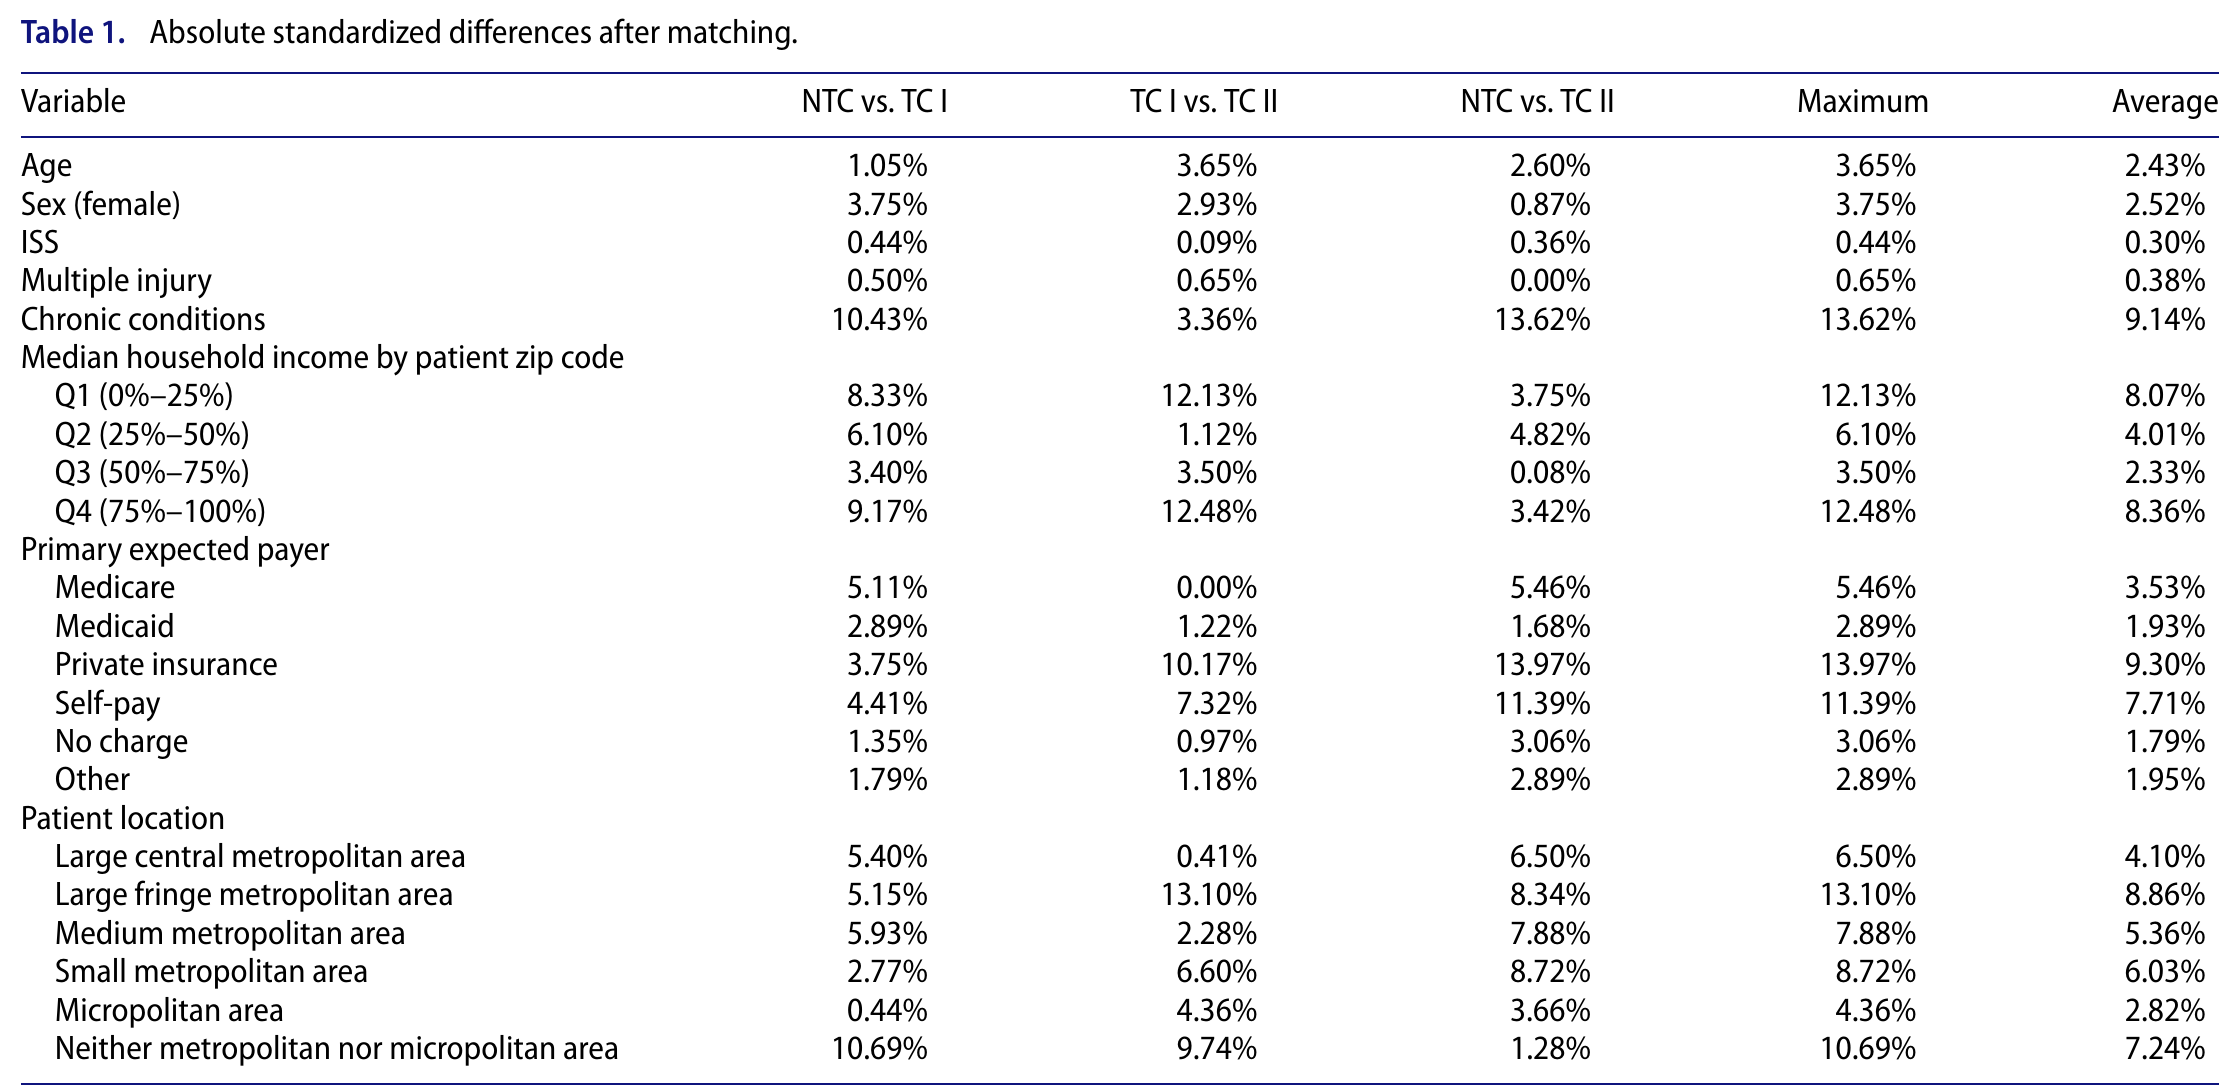
\includegraphics[width=\textwidth]{figures/nattino-table1.png}
    % \caption{\label{fig:label} }
  \end{figure}


  
\end{frame}

% -------------------------------------------------------------------------

\begin{frame}
  \frametitle{Results: Comparisons between trauma centers}

  \begin{figure}[ht]
    \centering
    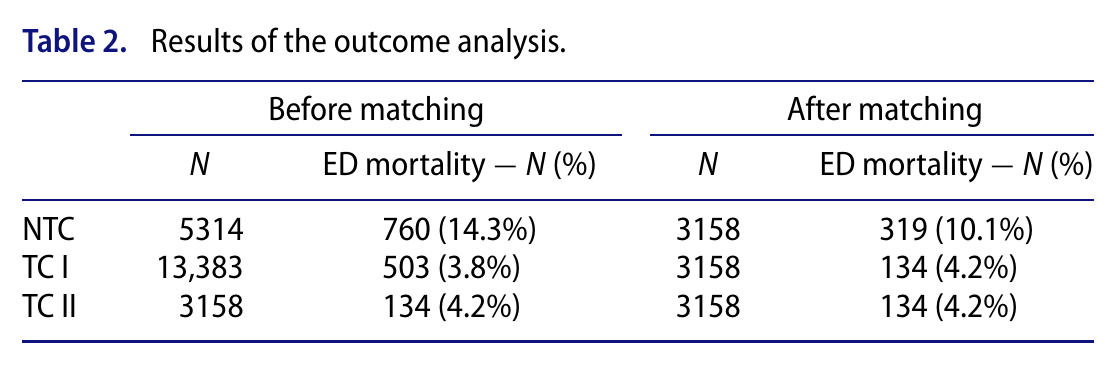
\includegraphics[width=0.7\textwidth]{figures/nattino-table2.png}
    % \caption{\label{fig:label} }
  \end{figure}

  \begin{itemize}
  \item NTC vs TC (TC I and TC II combined): $T_\text{MH}=11.45$, $p<0.001$ \medskip 
  \item TC I vs TC II: $T_\text{MN} = 0$, $p = 0.500$ \medskip 
  \item Assess sensitivity to unobserved confounding
    \citep{rosenbaum1987} gives $\Gamma_{\text{MH}} = 2.34$.
  \end{itemize}
  
\end{frame}

% -------------------------------------------------------------------------

% \begin{frame}
%   \frametitle{Sensiti}
  

  
  
  
% \end{frame}

%%% Local Variables:
%%% mode: latex
%%% TeX-master: "../main"
%%% End:


\section{S\"avje et al. (2017)}

% -------------------------------------------------------------------------

\begin{frame}
  \frametitle{S\"avje et al (2017)}
  
  \begin{itemize}
  \item \textbf{Hypothesis:} social norms influence citizens'
    propensity to vote \citep*{gerber2008social}.
  \item \textbf{Goal:} study effectiveness of a postcard intervention
    in increasing voter turnout.  There are six total treatment conditions. 
  \item Introduce \emph{generalized full matching}, which extends full
    matching to the case of categorical treatment with $k$ levels.
  \end{itemize}
  
  \medskip

  Gerber et al. prescreened voters to be included in the study, so the
  original results were not generalizeable to the entire population.
    
\end{frame}

% -------------------------------------------------------------------------

\begin{frame}
  \frametitle{Full matching}
  
  This paper generalizes full
  matching\footnote{\cite{rosenbaum2001,hansen2004,stuart2008}}: \medskip
  
  \begin{itemize}
  \item Construct groups of units that are as homogeneous as possible \medskip 
  \item Require that each group has at least one unit of each
    treatment condition \medskip
  \item So far, only developed for case of binary treatment
  \end{itemize}


  \bigskip

  \emph{All units} are matched to a subclass, hence the term ``full''

\end{frame}

% -------------------------------------------------------------------------

\begin{frame}
  \frametitle{Notation}
  
  \begin{itemize}
  \item Denote the sample of $n$ units by $\U = \{1,2,\ldots,n\}$    \medskip 
  \item Unit $i$ is assigned to treatment condition
    $W_i \in \{1,2,\ldots,k\}$ \medskip 
  \item The vectors $\w_x = \{i : W_i = x\}$ denote sets of units
    assigned to a given treatment condition \medskip 
  \item Matched groups are denoted by $\m$, and the union of matched
    groups is $\M = \{\w_1, \w_2, \ldots \}$ \medskip 
  \item Define an objective function
    $L: \mathcal{M} \rightarrow \mathbb{R}$, where $\mathcal{M}$ is
    the set of possible matches
  \end{itemize}


\end{frame}

% -------------------------------------------------------------------------

\begin{frame}
  \frametitle{Match group constraints}

  Constrain the set of admissible matches $\mathcal{M}$ as follows:

  \medskip 

  \begin{itemize}
  \item Each match group $\m$ must contain $c_x$ no. of units with
    treatment condition $x$ \medskip 
  \item Each match group must contain at least $t \geq \sum_{x=1}^{k}
    c_x$ no. of units overall \medskip 
  \item Union of match groups must contain all units, $\M = \bigcup \m = \U$
  \end{itemize}
  
\end{frame}

% -------------------------------------------------------------------------

\begin{frame}
  \frametitle{Algorithm}
  
  \ldots
  
\end{frame}


% -------------------------------------------------------------------------

\begin{frame}
  \frametitle{Graphical example}
  
  \begin{figure}[ht]
    \centering
    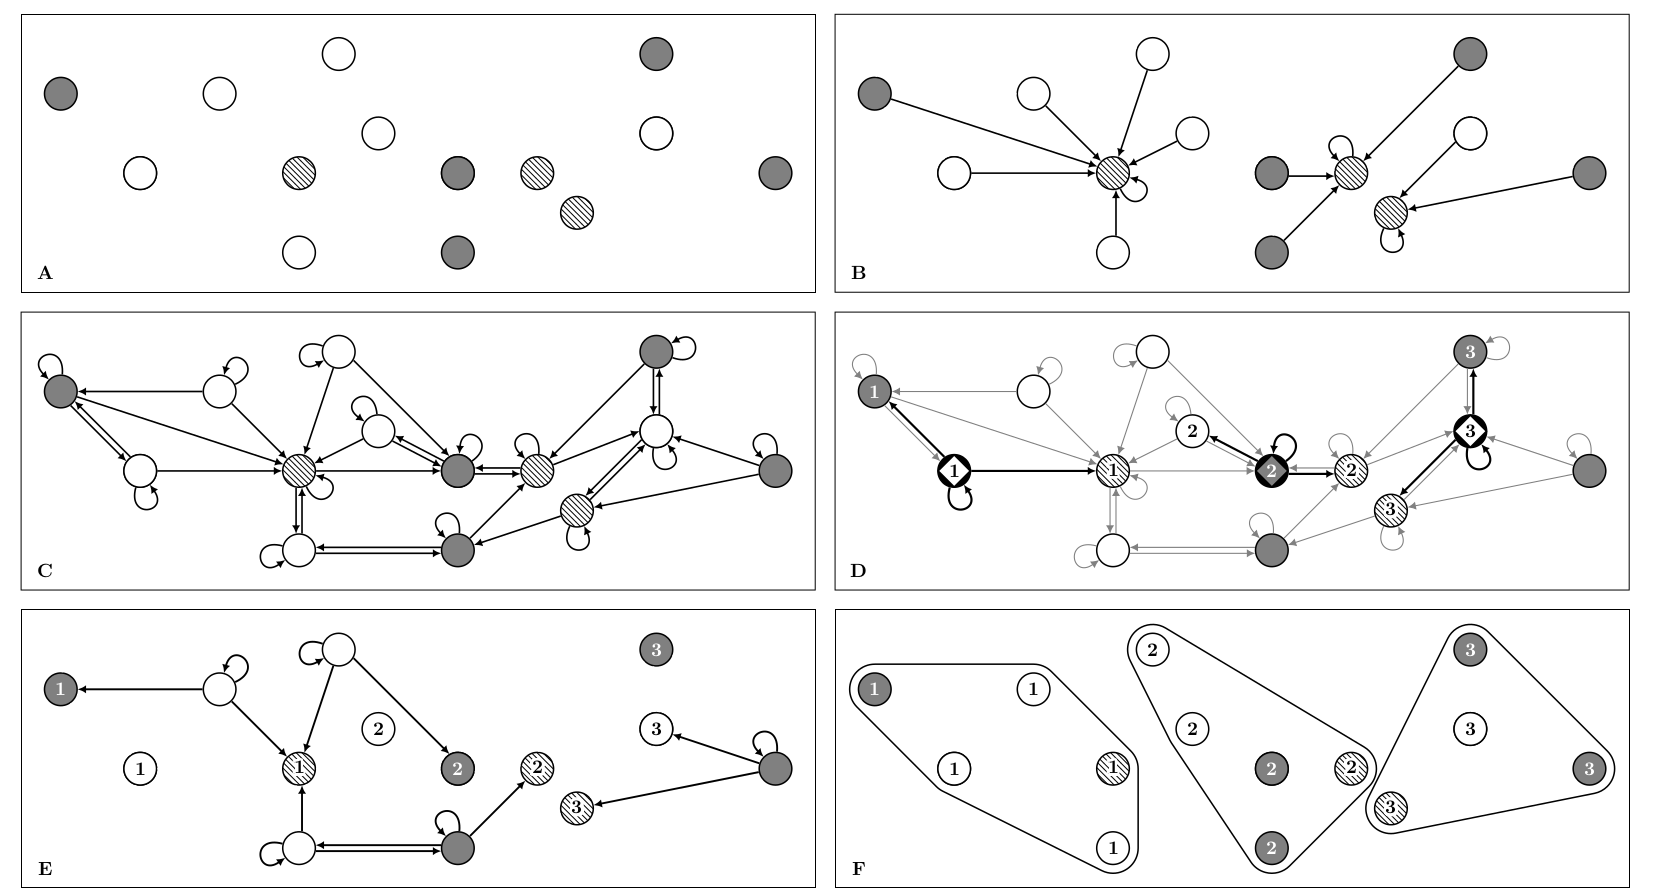
\includegraphics[width=\textwidth]{figures/saevje-network.png}
    % \caption{\label{fig:label} }
  \end{figure}

  
\end{frame}

% -------------------------------------------------------------------------

\begin{frame}
  \frametitle{Properties}

  Let $\M_{\text{alg}}$ be the set of matches resulting from the algorithm

  \begin{block}{Theorem: S\"avje et al. (2019)}
    $$L(\M_\text{alg}) \leq \min_{\M \in \mathcal{M}} 4 L(\M)$$
  \end{block}
  
\end{frame}

% -------------------------------------------------------------------------

\begin{frame}
  \frametitle{Covariate balance}
  
  \begin{figure}[ht]    
    \centering
    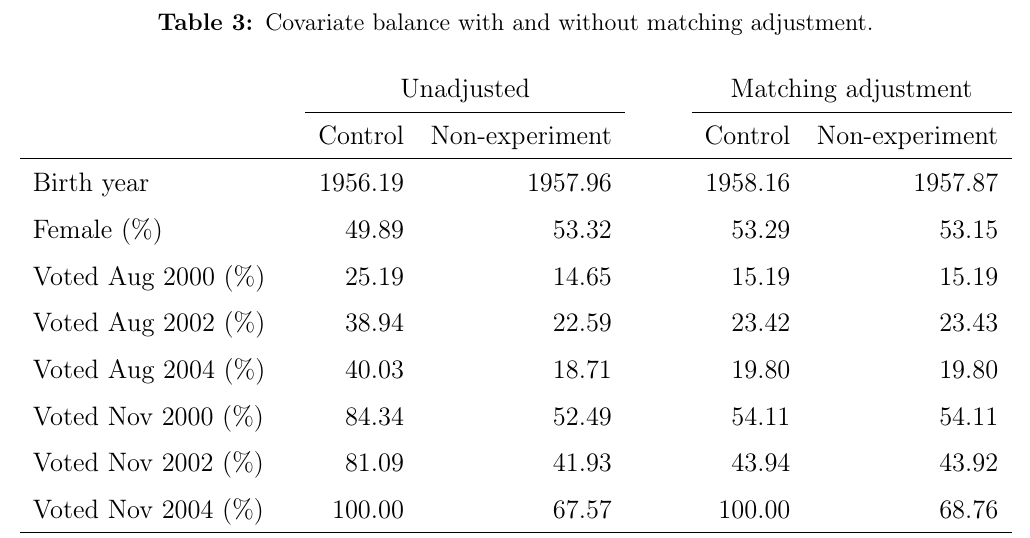
\includegraphics[width=0.99\textwidth]{figures/saevje-table3.png}
    % \caption{\label{fig:label} }
  \end{figure}

  Construct matched groups based on Mahalonobis distance
  
\end{frame}

% -------------------------------------------------------------------------



\begin{frame}
  \frametitle{Results on voter turnout data (1)}
  
  \begin{figure}[ht]    
    \centering
    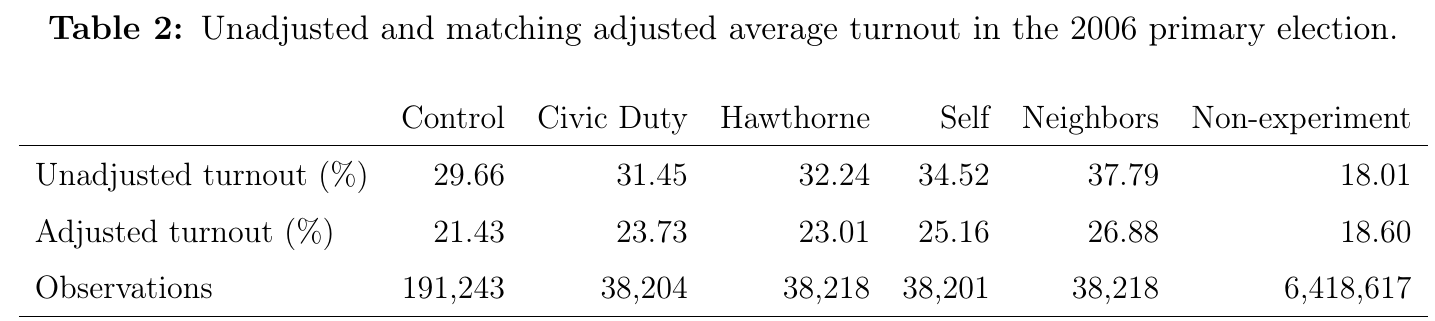
\includegraphics[width=0.99\textwidth]{figures/saevje-table2.png}
    % \caption{\label{fig:label} }
  \end{figure}

  \footnotesize{\emph{The figures [in the second row] should be
      interpreted as estimates of turnout of the six conditions if
      scaled up to the whole population}}

  \normalsize

  \medskip 

  Control and non-experiment groups should be more similar....
  
\end{frame}

% -------------------------------------------------------------------------

\begin{frame}
  \frametitle{Results on voter turnout data (2)}

  Now restrict to units that voted in 2004 election\ldots

  \medskip 

  \begin{figure}[ht]    
    \centering
    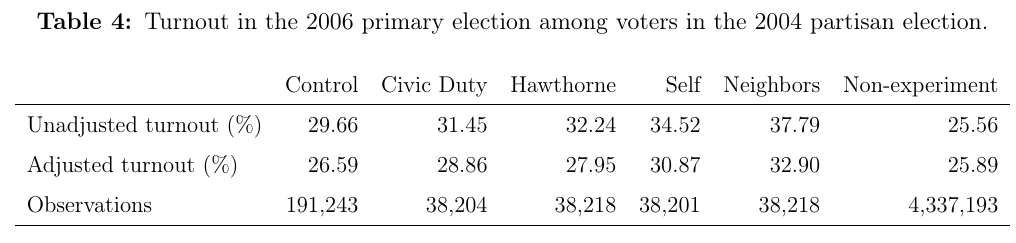
\includegraphics[width=0.99\textwidth]{figures/saevje-table4.png}
    % \caption{\label{fig:label} }
  \end{figure}


\end{frame}



% -------------------------------------------------------------------------

\begin{frame}
  \frametitle{Differences between Nattino et al. and S\"avje et al. }
  
  \begin{itemize}
  \item Nattio et al. \medskip 
    \begin{itemize}
    \item Attempt to mimic block randomization design \medskip 
    \item Adapts existing matched pair algorithm \medskip 
    \item Fisher randomization paradigm \medskip 
    \item Frequentist test and confidence intervals are standard \medskip 
    \end{itemize}
  \item S\"avje et al. \medskip 
    \begin{itemize}
    \item Less conventional experimental design $\rightarrow$ more
      researcher degrees of freedom (how to set $c_x$?) \medskip 
    \item Novel algorithm which generalizes full matching \medskip 
    \item Direct comparison of average outcomes \medskip 
    \item Quantifying uncertainty appears difficult, and is not
      attempted by the authors
    \end{itemize}
  \end{itemize}
  
\end{frame}


%%% Local Variables
%%% Local Variables:
%%% mode: latex
%%% TeX-master: "../main"
%%% End:


\section{Wu et al. (2020)}

% -------------------------------------------------------------------------

\begin{frame}
  \frametitle{Wu et al. (2020)}
  
  \begin{itemize}
  \item \textbf{Goal:} Study effect of long-term PM$_\text{2.5}$
    exposure on mortality rates \medskip 
  \item Estimand: $\E[Y(w)]$, where $Y$ is mortality rate per 100
    Medicare enrollees, and $w$ is PM$_\text{2.5}$ exposure in
    {\textmu}g/m$^\text{3}$
  \end{itemize}
  
\end{frame}

% -------------------------------------------------------------------------

\begin{frame}
  \frametitle{Local weak unconfoundedness}

  Treatment $W_j$ and covariates $\mathbf{C}_j$ \medskip 
  

    \begin{block}{\textit{Assumption}: Local weak unconfoundedness (Imbens, 2000)}
      $W_j \ind Y_j(w) \mid \mathbf{C}_j$ for all $w \in \mathcal{W}$ \smallskip

    \footnotesize \emph{Note: does not require joint independence of all
      potential outcomes $\{Y_j(w)\}_{w\in \mathcal{W}}$} \normalsize
  \end{block}

  Define the indicator variable $I_j(\tilde w) = 1$ if
  $W_j = \tilde w$ and $0$ otherwise.
  \begin{block}{\textit{Assumption}: Local weak unconfoundedness (Wu et al.)}
    $\{I_j(\tilde w)\}_{\tilde w \in [w-\delta, w+\delta]} \ind Y_j(w)
    \mid \mathbf{C}_j$ for all $z \in \mathcal{Z}$ \smallskip

    \footnotesize \emph{Note: this does not require joint independence of all
      potential outcomes $\{Y(z)\}_{z\in \mathcal{Z}}$} \normalsize
  \end{block}
  That is, the assignment is unconfounded \emph{within a neighborhood}
  of $w$ (not all $w \in \mathcal{W}$)

  \medskip Here $\delta$ is called the \textit{caliper}. 
  
\end{frame}

% -------------------------------------------------------------------------

\begin{frame}
  \frametitle{Matching with continuous treatments}
  
  \begin{itemize}
  \item Define a grid of values for $w$ \medskip 
  \item \textbf{Idea}: Match on both $w$ and the estimated GPS $e$,
    i.e. the objective function for matching is
    \begin{align*}
      m(e_j, w) = \arg \min_{k: w_k \in [w - \delta, w + \delta]}
      \| \lambda \cdot [e^\star(w_k, \mathbf{c}_k) - e^\star_j] +
      (1-\lambda) \cdot [w^\star_k - w^\star_j]\|
    \end{align*}
  \item The counterfactual outcome for unit $j$ at level treatment
    level $w$ is imputed as
    $\hat Y_j(w) = Y^{\text{obs}}_{m(e(w, \mathbf{c}_j), w)}$, i.e.,
    impute it from the unit close to $w$ (not $w_j$) and close in
    propensity score for unit $j$, $e_j$ \medskip
  \item Must select tuning parameters $\lambda$ and $\delta$ \medskip 
  \item Take average within each level of $w$, then use a kernel
    smoother to estimate the dose-response curve
  \end{itemize}


  
\end{frame}

% -------------------------------------------------------------------------

\begin{frame}
  \frametitle{Results on PM$_\text{2.5}$ mortality data} 
  
  \begin{figure}[ht]
    \centering
    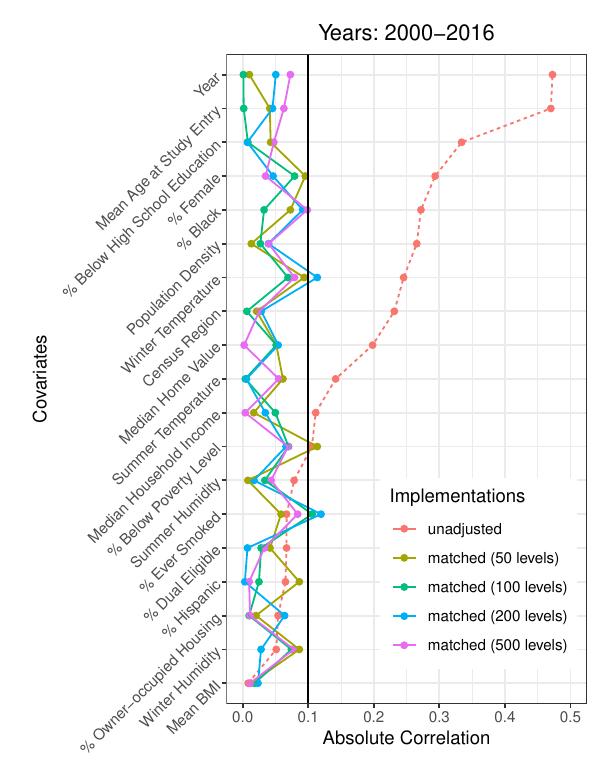
\includegraphics[height=0.8\textheight]{figures/wu-fig2.png}
  \end{figure}

  
\end{frame}

% -------------------------------------------------------------------------

\begin{frame}
  \frametitle{Results on PM$_\text{2.5}$ mortality data} 
  
  \begin{figure}[ht]
    \centering
    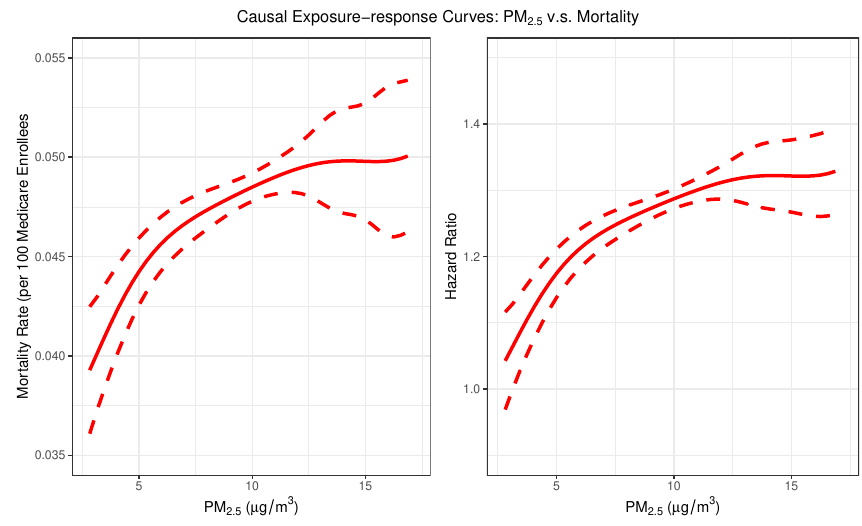
\includegraphics[width=\textwidth]{figures/wu-fig3.png}
  \end{figure}

  Confidence bands
  
\end{frame}


% -------------------------------------------------------------------------



\begin{frame}
  \frametitle{Open questions from Wu et al.}
  
  \begin{itemize}
  \item Is the bootstrap a valid way to represent uncertainty? \medskip 
  \item This method cannot estimate heterogeneous effects (e.g.,
    subgroups of the population)
  \end{itemize}
  
\end{frame}

%%% Local Variables:
%%% mode: latex
%%% TeX-master: "../main"
%%% End:

\AtBeginSection[]{
}


\section{Conclusion}

% -------------------------------------------------------------------------

% \begin{frame}
%   \frametitle{Conclusion}
  
%   \begin{itemize}
%   \item Nattino et al. (2020)
%     \begin{itemize}
%     \item \textbf{Pros:}
%     \item \textbf{Cons:} 
%     \end{itemize}
%   \item S et al. (2020)
%     \begin{itemize}
%     \item \textbf{Pros:}
%     \item \textbf{Cons:} 
%     \end{itemize}
%   \item Nattino et al. (2020)
%     \begin{itemize}
%     \item \textbf{Pros:}
%     \item \textbf{Cons:} 
%     \end{itemize}

%   \end{itemize}
  
% \end{frame}

% -------------------------------------------------------------------------

\begin{frame}
  \frametitle{Conclusion}
  
  Slides at \textcolor{dodgerblue3}{\texttt{spencerwoody.github.io/talks}}
  
\end{frame}

%%% Local Variables:
%%% mode: latex
%%% TeX-master: "../main"
%%% End:


% Now 


% Sections
% \input{input/formatting}

% -------------------------------------------------------------------------

% Bibliography
\begin{frame}[t,allowframebreaks]
\frametitle{References}


\begingroup
\renewcommand{\section}[2]{}
\tiny
\bibliography{main}
\endgroup
\normalsize

\end{frame}

\appendix
\backupbegin

% -------------------------------------------------------------------------
% Extra slides

% \frame{Extra slides...}

% And your backup slides here
% \frame{\lipsum[3]}
\backupend



\end{document}

%%% Local Variables:
%%% mode: latex
%%% TeX-master: t
%%% End:
